% ------------------------------------------------------------------
\renewcommand{\thisweek}{MATH327 Week 3}
\renewcommand{\moddate}{Last modified 13 Feb.~2021}
\setcounter{section}{3}
\setcounter{subsection}{0}
\phantomsection
\addcontentsline{toc}{section}{Week 3: Canonical ensemble}
\section*{Week 3: Canonical ensemble}

\subsection{The thermal reservoir}
\subsubsection{Replicas and occupation numbers}
While it is relatively easy to prevent particle exchange, for example by sealing gases inside airtight containers, it is not practical to forbid energy exchange as would be needed to fully isolate statistical systems.
Any thermal insulator is imperfect, and even in the deepest reaches of space we would still be bombarded by cosmic microwave radiation.
In practice it is more convenient to work with physical systems that are characterized by their (intensive) temperatures rather than their (extensive) internal energies.

\begin{shaded}
  This leads us to define a \textbf{canonical ensemble} to be a statistical ensemble characterized by its fixed temperature $T$ and conserved particle number $N$, with the temperature held fixed through immersion in a \textbf{thermal reservoir}.
\end{shaded}

The second part of this definition connects the fixed temperature to the fundamental fact of energy conservation (the first law of thermodynamics).
This is done by proposing that our system of interest \Om is in thermal contact with a much larger external system $\Om_{\text{res}}$---the thermal reservoir, sometimes called a ``heat bath''.
The overall combined system $\Om_{\text{tot}} = \Om_{\text{res}} \otimes \Om$ is governed by the micro-canonical ensemble, with conserved total energy $E_{\text{tot}} = E_{\text{res}} + E \approx E_{\text{res}}$, while the energy $E$ of \Om is allowed to fluctuate.
The key qualitative idea is that, in thermodynamic equilibrium, \Om has a negligible effect on the overall system.
In particular, the temperature of that overall system---and therefore the temperature of $\Om$, by intensivity---is set by the reservoir and remains fixed even as $E$ is allowed to fluctuate by energy exchange.
This effectively generalizes the setup we used to analyze heat exchange last week, where we saw that thermal contact causes a new flow of energy from hotter systems to colder systems, cooling the former by heating the latter.

The mathematical realization of this argument, as developed by Gibbs, proceeds by taking $\Om_{\text{tot}}$ to consist of many ($R \gg 1$) identical \textbf{replicas} of the system \Om that we're interested in.
All of these replicas are in thermal contact with each other, and in thermodynamic equilibrium.\footnote{The thermal contact between any two replicas can be indirect, mediated by a sequence of intermediate replicas.  This transitivity of thermodynamic equilibrium is sometimes called the \href{https://en.wikipedia.org/wiki/Zeroth_law_of_thermodynamics}{zeroth law of thermodynamics}.  It declares that if systems $\Om_A$ \& $\Om_B$ are in thermodynamic equilibrium while systems $\Om_B$ \& $\Om_C$ are in thermodynamic equilibrium, then $\Om_A$ \& $\Om_C$ must also be in thermodynamic equilibrium.}
Choosing one of the subsystems to be the \Om we consider, the other $R - 1 \gg 1$ replicas provide the thermal reservoir $\Om_{\text{res}}$.

An extremely small example of this setup is illustrated by the figures below.
We take each subsystem to consist of only $N = 2$ spins.
For now we assume the spins are \textit{distinguishable}, so that $\downarrow\uparrow$ and $\uparrow\downarrow$ are both distinct micro-states.
This means that each individual subsystem has only the $M = 4$ micro-states $\om_i$ defined below.
\begin{center}
  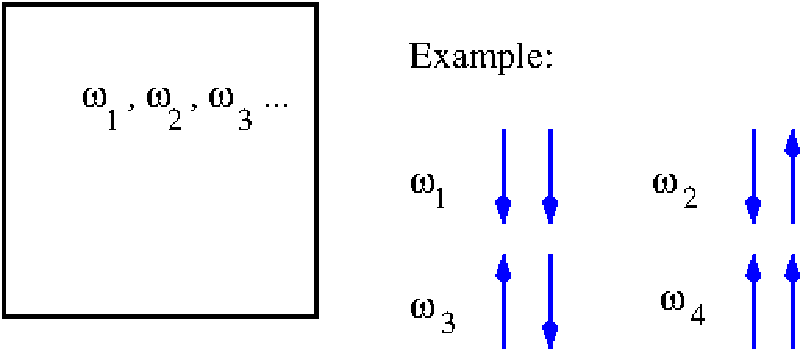
\includegraphics[width=0.7\textwidth]{figs/week03_spin-system.pdf}
\end{center}
To form the overall system $\Om_{\text{tot}}$ we now bring together the $R = 9$ replica subsystems shown below.
We draw boxes around each replica to remind us that they are allowed to exchange only energy with each other, while the $N = 2$ spins are conserved in each subsystem.
We pick out one of these replicas (coloured red) to serve as the system \Om we will consider.
The other $8$ are the thermal reservoir $\Om_{\text{res}}$ that fixes the temperature of $\Om$.
\begin{center}
  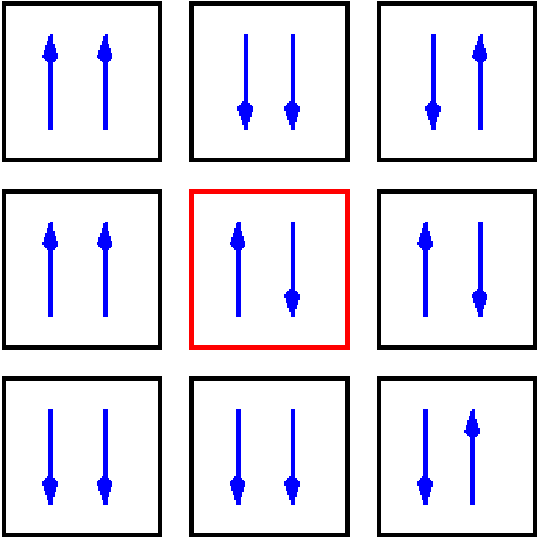
\includegraphics[width=0.7\textwidth]{figs/week03_spin-reservoir.pdf}
\end{center}

A convenient way to analyze the overall system of $R$ replicas is to define the \textbf{occupation number} $n_i$ to be the number of replicas that adopt the subsystem micro-state $\om_i$ in any given micro-state of the overall system.
The index $i \in \left\{1, 2, \cdots, M\right\}$ runs over all $M$ subsystem micro-states.
In the example above, three of the replicas in the second figure have the micro-state $\om_1 = \downarrow\downarrow$, meaning $n_1 = 3$.
What are the occupation numbers $\left\{n_2, n_3, n_4\right\}$ for the other three $\om_i$ in the figures above?
Are all replicas are accounted for, $\sum_i n_i = R$?
\begin{mdframed}
  \ \\[50 pt]
\end{mdframed}
Normalizing the occupation number by $R$ gives us a well-defined \textit{occupation probability}, $p_i = n_i / R$ with $\sum_i p_i = 1$.
This $p_i$ is the probability that if we choose a replica at random it will be in micro-state $\om_i$.

Now let us consider conservation of energy, which continues to apply to the total energy $E_{\text{tot}}$ of the overall system $\Om_{\text{tot}}$.
We assume that each replica's energy $E_r$ is independent of all the other replicas.
(This is guaranteed for the non-interacting systems we will focus on until week 10, and also holds when interactions are allowed within each replica but not between different replicas.)
The thermal contact between replicas allows $E_r$ to fluctuate (subject to conservation of $E_{\text{tot}}$), but there are at most $M$ values $E_i$ it can take, one for each of the $M$ subsystem micro-states $\om_i$.
This allows us to rearrange a sum over replicas into a sum over subsystem micro-states:
\begin{equation}
  \label{eq:canon_Etot}
  E_{\text{tot}} = \sum_{r = 1}^R E_r = \sum_{i = 1}^M n_i E_i,
\end{equation}
with $E_i$ the energy of a replica in micro-state $\om_i$ and the occupation number $n_i$ counting how many times this micro-state appears in the sum over the $R$ replicas.
(We can assume that $R$ and $M$ are both finite, so we don't need to worry about rearranging infinite sums.)
% ------------------------------------------------------------------



% ------------------------------------------------------------------
\subsubsection{Partition function}
Following Gibbs, we have already simplified the mathematics by specializing to the case in which the thermal reservoir consists of $R - 1$ replicas of the (sub)system of interest, $\Om$, all in thermodynamic equilibrium.
The next step is to further specialize to consider only a fixed set of occupation numbers $n_i$.
From \eq{eq:canon_Etot}, we see that this is essentially equivalent to considering \Om whose micro-states all have unique energies, $E_i \ne E_j$ for any $\om_i \ne \om_j$.
We also see that this guarantees the total energy $E_{\text{tot}}$ is conserved, allowing us to apply the micro-canonical tools we developed last week to the overall $\Om_{\text{tot}}$.
The results we obtain will continue to hold for more general situations where the conserved $E_{\text{tot}}$ could correspond to multiple different sets of occupation numbers, for which the mathematics is more complicated.

Based on the conservation of $E_{\text{tot}}$, we want to determine the temperature of $\Om_{\text{tot}}$, which fixes the temperature of the single subsystem of interest, $\Om$.
According to our work last week, to do this we first need to compute the overall number of micro-states $M_{\text{tot}}$ for a given $E_{\text{tot}}$, from which we can derive the entropy and temperature since the system is in thermodynamic equilibrium.
By fixing the occupation numbers $n_i$, we already know how many times each micro-state $\om_i$ appears among the $R$ replicas.
To determine $M_{\text{tot}}$ we just need to count how many possible ways there are of distributing the $\left\{n_i\right\}$ micro-states among the $R$ replicas.

If we consider first the micro-state $\om_1$, the number of possible ways of distributing $n_1$ copies of this micro-states among the $R$ replicas is just the binomial coefficient
\begin{equation*}
  \binom{R}{n_1} = \frac{R!}{n_1! \; (R - n_1)!}.
\end{equation*}
Moving on to $\om_2$, we need to keep in mind that $n_1$ replicas have already been assigned micro-state $\om_1$, so there are only $R - n_1$ replicas left to choose from, implying
\begin{equation*}
  \binom{R - n_1}{n_2} = \frac{(R - n_1)!}{n_2! \; (R - n_1 - n_2)!}.
\end{equation*}
possibilities.
Repeating this process for all micro-states $\left\{\om_1, \om_2, \cdots, \om_M\right\}$, we obtain the telescoping product
\begin{equation*}
  \begin{split}
    M_{\text{tot}} & = \binom{R}{n_1} \binom{R - n_1}{n_2} \cdots = \frac{R!}{n_1! \; (R - n_1)!} \frac{(R - n_1)!}{n_2! \; (R - n_1 - n_2)!} \cdots \\
                   & = \frac{R!}{n_1! \; n_2! \; \cdots \; n_M!},
  \end{split}
\end{equation*}
since $\left(R - \sum_i n_i \right)! = 0! = 1$.
From this we can see that the order in which we assign micro-states to replicas is irrelevant, since integer multiplication is commutative.

Thanks to thermodynamic equilibrium, the entropy is
\begin{equation*}
  S(E_{\text{tot}}) = \log M_{\text{tot}} = \log(R!) - \sum_{i = 1}^M \log(n_i!),
\end{equation*}
where the dependence on $E_{\text{tot}}$ enters through the occupation numbers via \eq{eq:canon_Etot}.
Assuming that both $R \gg 1$ and every occupation number $n_i \gg 1$, we can approximate all of these logarithms using Stirling's formula,
\begin{align*}
  \log(N!) & = N \log N - N + \cO(\log N) \approx N \log N - N &
  \mbox{for } N & \gg 1.
\end{align*}
Back in \eq{eq:CLT_states} we used the central limit theorem to derive a form of this approximation that included the leading $\log N$ terms we neglect here.
Note that $n_i \gg 1$ for all $1 \leq i \leq M$ implies that the number of replicas is much larger than the number of micro-states for a single subsystem, $R \gg M$.
As we have discussed before, the number of micro-states $M$ is typically a very large number, so the thermal reservoirs we are formally considering must be truly enormous!

\newpage % WARNING: FORMATTING BY HAND
Applying the approximation above, what do you find for $S(E_{\text{tot}})$ in terms of $R$ and $n_i$?
Replacing $n_i = R p_i$, what is the entropy in terms of the occupation probabilities?
\begin{mdframed}
  \ \\[100 pt]
\end{mdframed}

In your result, the dependence on $E_{\text{tot}}$ now enters through the occupation probabilities $p_i$.
In order to make the energy dependence explicit and determine the temperature, we have to express $p_i$ in terms of $E_{\text{tot}}$.
We do this by applying our knowledge from last week that thermodynamic equilibrium implies maximal entropy.
In the maximization, there are now two constraints that we will need to include through two Lagrange multipliers: $\sum_i p_i = 1$ and $\sum_i n_i E_i = E_{\text{tot}}$ (\eq{eq:canon_Etot}).
Writing everything in terms of occupation probabilities we therefore need to maximize the modified entropy
\begin{equation*}
  \Sbar = -N \sum_{i = 1}^M p_i \log p_i + \al\left(\sum_{i = 1}^M p_i - 1\right) - \be\left(R \sum_{i = 1}^M p_i E_i - E\right)
\end{equation*}

\TODO{Being written...}
% ------------------------------------------------------------------



% ------------------------------------------------------------------
\newpage % TODO: Placeholder...
\subsection{Internal energy and heat capacity}
\TODO{Being written...}
% ------------------------------------------------------------------



% ------------------------------------------------------------------
\newpage % TODO: Placeholder...
\subsection{Helmholtz free energy}
\TODO{Being written...}
% ------------------------------------------------------------------



% ------------------------------------------------------------------
\newpage % TODO: Placeholder...
\subsection{Distinguishable Spins}
\TODO{Being written...}
% ------------------------------------------------------------------



% ------------------------------------------------------------------
\newpage % TODO: Placeholder...
\subsection{Indistinguishable Spins}
\TODO{Being written...}
% ------------------------------------------------------------------
